
\subsubsection{Abstract}
%%% Lukas: this got pretty long now
We replicated the model described by Rafferty et al. to optimize automated teaching via POMDP planning. 

Teaching is formulated as a partially observable Markov decision process (POMDP) in which the teacher operates and plans on the belief state which maps to the student's knowledge state.
The automated teacher employs a cognitive learner model that defines how the student's knowledge state changes assuming a Bayesian belief update.

Two concept learning tasks are considered to evaluate the algorithm: (i) a simple \textit{letter arithmetic} task for which the goal is to find the correct mapping between a set of letters and numbers, (ii) a \textit{number game}, in which students need to learn which number concept is the target (e.g. is the rule used for generating the items 'odd numbers' or 'numbers between 15-25'?)

Three learner models were postulated: a memoryless model that stochastically chooses a matching concept based on the current action, a discrete model with memory that additionally matches concepts with previously seen actions and a continuous model with a probability distribution over all concepts that eliminates inconsistent concepts based on the actions.

We implemented all models and both tasks, and ran simulations following the same protocol as the original paper. We were able to replicate all three models for the first task with comparable results. In the second task, our results differ in minor ways which leads to a different evaluation of the models. % i.e. MIG is still pretty good
%%% Lukas: does it make sense to write this here already?
While the POMDP models outperform the random baselines overall, an advantage over the policy based on maximum information gain can not be clearly seen.

% Note that no human experiments were conducted to evaluate the models.

We open source our implementation in Python and extend the description of the learner models with explicit formulas for the belief update, as well as an extended description of the planning algorithm, hoping that this will help other researchers to extend this work.

\section{Introduction}

% TODO Citations are missing
% The increasing digitalization of teaching and learning activities is changing how students gather new knowledge. Electronic applications can easily be used to learn certain topics such as languages. A lot of effort has been put into creating useful applications and developing strategies to teach material without a real teacher. Such human teachers have the ability to form hypothesis about the students' level of knowledge and understanding of a certain topic and they can adjust their approach on the fly to better fit the learners' status. She might notice that certain methods are not effective for some students and choose a different method, or is able to progress faster through a set of concepts if she notices that this is already well understood.
%This level of understanding of the students' knowledge and a consequential ability to adjust the teaching activities is mostly lacking in digital teaching applications. As personalization and adaptation are increasingly becoming important, this is yet an area where this has to be successfully applied.

Teaching students in an automated fashion is a challenging task. Human teachers are able to adjust the teaching process to the students depending on their current situation (e.g. a teacher will act differently if he thinks that the student didn't fully understand a concept yet, or if he already mastered it). This level of understanding of the student's knowledge and a consequential ability to adjust the teaching activities is not straightforward in automated teaching applications.

One method for increasing the teaching effectiveness in automated teaching applications was proposed by Rafferty \textit{et al.}~\cite{rafferty2016faster}\footnote{Note that there is a shorter version with the same method described which only contains the first task of this longer paper. We always refer to the longer and later paper in this replication.}. They model teaching as a partially observable Markov decision process (POMDP), considering the selection of the next teaching activity as a planning problem. The automated teacher employs a cognitive learner model that defines how the student's knowledge state is expected to behave and that defines how the internal belief update is calculated.

As the title of the paper suggests, the goal of the teacher is to teach the student quickly. The teaching activities have a time cost associated and the goal is to minimize the total time until a concept is learned. 

The teacher has three types of teaching activities available: showing an example (i.e. teaching new content), asking a quiz (i.e. assessing the knowledge of the student), and a question with feedback action (i.e. a question is asked and the question's correct answer is then revealed).

Three models of the learner, each one with a different complexity, are proposed: a memoryless model, a discrete model with memory and a model with a continuous knowledge state. 
% TODO extend?

The combination of learner model and teaching action defines the belief update computation. During the planning phase, a set of sample actions are evaluated by a tree search algorithm with limited horizon, where the belief is simulated according to the learner model. The teacher selects the action which is expected to bring the student the closest to the desired knowledge at the lowest cost.
% TODO cannot optimize for both, note it correctly here?

The algorithm is evaluated on two concept learning tasks: (i) a simple \textit{letter arithmetic} task with the goal of finding the correct mapping between a set of letters and numbers, (ii) a \textit{number game}, in which students need to learn which number concept is the target (e.g. is the rule used for generating $x$ 'odd numbers' or 'numbers between 15-25'). 


%%% Lukas: not sure, hard to compare with original version
% TODO re-check
We reimplemented the algorithms and we evaluated our implementation through the same simulations as in the original work, and achieved overall comparable results.
Our results differ slightly though that the policy based on maximum information gain still achieves overall comparable results to the learner models with estimation based on learning. 
% TODO: re-evaluate?
In the first task, the process performs well, however, the different models perform very similar with a sophisticated student and are not better than a baseline based on maximum-information gain. 
In the second task (more complex), the POMDP teacher was able to teach better than the baseline. However, no single learner model was clearly better than the others.
% Nevertheless, we would consider the maximum information gain policy a valid POMDP policy as it employs the continuous belief model.
% There are some weaknesses in the formulation but it is still an interesting approach to the teaching problem.


% check
Our implementation is open and can be found at https://github.com/luksurious/faster-teaching.

%This work replicates the algorithm from the original paper to provide a freely available implementation in Python for the research community. 
% We extend the description of the learner models with explicit formulas for the belief update %and understanding of the method, which the original paper may have lacked in some areas
% and clarify details necessary for replicating them. 


\section{Methods}

\subsection{Teaching as a POMDP}

\subsubsection{General framework}

% Lukas: Do I need a source for this?

\begin{figure}
    \centering
    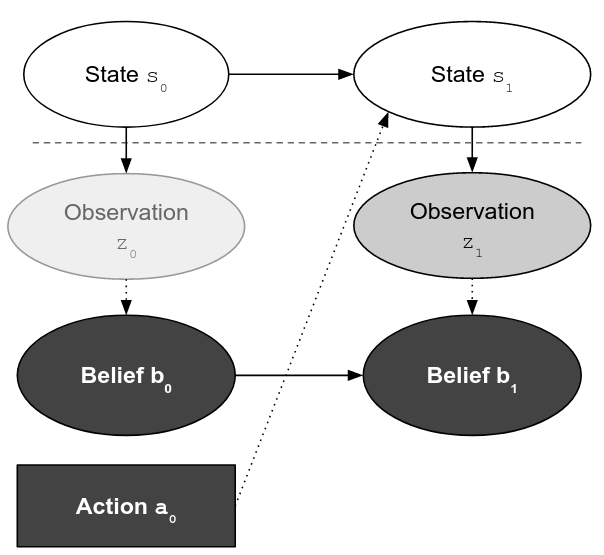
\includegraphics[width=0.5\linewidth]{pomdp-state.png}
    \caption{A general process of a POMDP. True states are not available, instead observations might be seen. This can be used to update the belief of the agent about the true state to help choose an action that would change the state and produce a new observation.}
    \label{fig:pomdp}
\end{figure}

% \begin{table}
%     \centering
%     \begin{tabular}{ll|l}
%         \hline
%         Set/Function         & Elements              & description  \\
%         \hline
%         $S$         & $s, s'$               & State of the environment \\
%         $A$         & $a$                   & Actions available to the agent \\
%         $R(s,a)$    & $r$                   & Reward function and resulting reward \\
%         --          & $\gamma \in [0,1]$    & Discount factor \\
%         $T(s'|s,a)$ & --                    & Conditional transition model \\
%         \hline
%         $Z$         & $z$                   & Set of observations about the environment/state \\
%         $O(o|s',a)$ & --                    & Conditional observation model \\
%         $B$         & $b, b'$               & Belief space and belief states \\
%         $\tau(b,a,z)$ & --                  & Belief update function \\
%         \hline
%     \end{tabular}
%     \caption{POMDP elements}
%     \label{tab:pomdp-elements}
% \end{table}

A partially observable Markov decision process (POMDP) extends a Markov decision process (MDP) such that the agent does not directly observe the state of the environment and instead receives (partial) observations of the state.
% Hence, it is composed of the elements of an MDP extended by the partial observability.

Similar to an MDP, the state space $S$ describes the state of the environment, the action space $A$ is the set of possible actions the agent can take, the reward function $R(s, a)=r$ describes the outcome for the agent after taking an action $a \in A$ in state $s \in S$, and the transition model $T(s'|s,a)$ describes the conditional probability of the environment transitioning from state $s \in S$ to state $s' \in S$ after the agent has taken action $a \in A$.
Finally, $\gamma \in [0,1]$ is a discount factor that describes how important future rewards are in comparison to immediate rewards when determining an optimal policy.

In a POMDP, as the states are not directly available to the agent, the set of possible observations of the environment are denoted $z \in Z$ and the conditional observation model $O(z|s',a)$ assigns a probability of receiving the observation $z$ after taking action $a$ causing a transition to $s'$.
% the observation space $Z$, 
% the transition model $p(s'|s,a)$, 
% the observation model $p(z|s,a)$, 
% the reward function $r(s,a)$, 
% and a discount factor $\gamma$. 
% In contrast to a regular MDP, in a POMDP, the true state is not available to the agent operating in the environment. 
To track the state of the environment, the agent maintains a probability distribution over the state space $S$ called the belief $b$.
% I don't find it useful to define the belief state $B$ ?
$b(s)$ then is the probability the agent assigns to the state $s$ matching the environment's state.

Through a series of observations, the agent is able to update this belief to infer the state of the environment.
The goal of the agent is to find an action sequence that maximizes the expected discounted future rewards $E\left[\sum_{t=0}^\infty \gamma^t r_t \right]$ where $t$ denotes the time step of the interaction and $r_t$ is the reward at that step. 

Figure \ref{fig:pomdp} describes the interaction in a POMDP. 
Taking an action $a_0 \in A$ causes a transition of the environment's state from $s_0$ to $s_1$ with probability $T(s'=s_1|s=s_0,a=a_0)$. 
Then, the agent receives the observation $z_1$ with probability $O(z=z_1|s'=s_1,a=a_0)$ and a reward $r_1=R(s=s_1,a=a_0)$ (not shown).
This enables the agent to update its belief from $b_0$ to $b_1$ as described in the next section.
% TODO find reference?
With a correct model of the environment and an intelligent agent, the probability of the correct state under the belief should increase $b_1(s_1) \geq b_0(s_0)$.

\subsubsection{Belief update}

We denote the operation of updating the belief $b'=\tau(b,a,z)$.
It depends only on the previous belief, the current action and the current observation because the state is assumed to be Markovian.

A generic belief update follows Bayesian statistics.
For discrete states, the probability of a single state can be updated using the formula:
\begin{equation}
    b'(s') = \eta \cdot O(z|s',a) \cdot \sum_{s \in S} T(s'|s,a) \cdot b(s)
    \label{eq:belief}
\end{equation}
where $\eta$ is a normalization term.
It is the inverted sum of the new belief state $1 / \sum_{s'} b'(s')$ as the probability distribution must sum up to $1$. 
This formula must be applied to every state $s \in S$ to obtain the updated belief $b'$.
The complexity of a full belief update is then of order $O(|S|^2)$.

\subsubsection{Application to automated teaching}

This formulation can be applied to automated teaching as follows: the student represents the environment and the knowledge of the student is modeled as the state $s \in S$ that is hidden from the teaching program.
The automated teacher is the agent operating in this environment by choosing actions $a \in A$ to teach the topic.
% \footnote{\textbf{POMDP action and teaching action.} 
%Both terms refer to the activity the teacher performs. In the POMDP framework, the action encompasses everything related to the action, i.e. also the content or item which is being taught. In the teaching framework, the action refers to the type of activity which can be applied to different teaching items. For example, the teaching action might be \textit{example} which is independent from \textit{what} is shown. In the context of the POMDP, the action refers to both the \textit{example} and the \textit{item}.
%, the automated teacher tries to change the student's state in such a way that he learns the correct concepts (goal state).
The student responds to actions with answers $z \in Z$ that represent the observations for the automated teacher.
The automated teacher maintains a belief $b$ as a probability distribution of the knowledge of the student.
Its goal is to change the state of the student, i.e. the knowledge, such that the student knows the topic.
The teacher employs a reward function according to the pedagogical objective(s).
We can simplify the reward function to only depend on the action $R(a)$.

If the student's learning behavior is known, the teacher is able to plan and choose actions in such a way that the learning of the student is optimized. 
Such a model would thus define the transition and observation functions needed to apply the POMDP framework.


Rafferty \textit{et al.} consider that an action $a$ is the choice of a specific type of \textit{teaching activity} $t \in T$ (type) \textit{and} a specific \textit{teaching item} $i \in I$ that describes some content or example of the topic.
This decomposition allows to simplify the formulation when different teaching methods are available.
See section \ref{sec:concept-learning} for more details.

\subsubsection{Planning optimal actions}

Finding a policy that optimizes the pedagogical objective(s) is done via online planning, i.e. during execution. Offline planning, i.e. precomputing best actions for every possible belief state, might become computationally expensive and, thus, not tractable for teaching tasks with a large state space or for longer trials. 
Hence, Rafferty \textit{et al.} employ a forward tree search algorithm with finite horizon similar to Ross \textit{et al.}~\cite{rossPomdp2008}.

The process in a nutshell is as follows:
The forward search starts from the current belief state $b$. 
A set of actions $\Tilde{A} \subset A$ is sampled to lower the computational cost.
Their values $q$ are calculated until horizon $d$ (depth) and the action $a^* \in A$ with the highest value is selected by the automated teacher.
Note that we follow the convention from reinforcement learning literature to denote state values with $V$ and state-action values with $Q$.

Thus, we compute the best action $a^*_d(b)$ as follows:
\begin{equation}
    a^*_d(b) = \arg \max_{a \in \Tilde{A}} Q_d(b, a)
    \label{eq:best-action}
\end{equation}
with $b$ the current belief state, $d \in \mathbb{Z}$ the search depth and $\Tilde{A} \subset A$ the sampled actions.

Since actions are composed of items $i \in I$ and teaching activity types $t \in T$, the action sampling is decomposed as follows:
$n$ teaching items $\Tilde{I} \subset I$ are sampled and the cartesian product of all available teaching activity types $T$ is constructed to create $\Tilde{A} = \Tilde{I} \times T$.
The number of sampled actions is then equal to the product of sampled items and number of teaching types $|\Tilde{A}| = n \cdot |T|$.
This prevents ending up with actions of only a few types, which is very probable in the case of $|I| >> |T|$.

A single action $a$ might cause different state changes according to $T(s'|s,a)$, and thus, different observations $z$.
For each action-observation pair, a new belief $b'=\tau(b,a,z)$ is computed.
With this new belief, the process starts anew: new actions are sampled and evaluated.
The forward search, thus, expands tree-like and grows exponentially in breadth.
If the set of possible observations following an action depends on the action or the teaching activity associated with the action, we can simplify the calculation by only considering those observations that are possible for that teaching activity $Z_{i_a} \subset Z$.

To calculate the value of an action under the current belief, the future expected values of all possible observations for that action need to be considered and added to the value of the action itself. 
We compute $Q_d(b, a)$, the expected value for using the action $a \in A$ in the belief $b$ with search depth $d$ as:

\begin{equation}
    Q_d(b, a) = \begin{cases}
        \Hat{V}(b) & \, \text{if $d$ = 0}\\
        R(a) + \sum_{z \in Z_{i_a}} Pr(z|b,a) \cdot \gamma \cdot V_{d-1}(b' = \tau(b, a, z)) & \, \text{otherwise}
    \end{cases}
\end{equation}
with
$\Hat{V}(b)$ an estimation function of the value of the belief $b$, 
$R(a)$ the expected reward for action $a$,
$Pr(z|b,a)$ the probability of receiving $z$ for action $a$ under the belief $b$,
$\gamma \in [0, 1]$ the discount factor, 
and $V_d(b')$ the value function for the new belief.
%The value functions carry the depth of the current recursion and if it becomes $0$, the value estimation of the belief is used instead of calculating it by enumeration.

The value of the belief $V_d(b)$ is then defined as the maximum value of the belief-action values $Q_d(b,a)$ for search depth $d$ of the sampled actions $\Tilde{A}$:
\begin{equation}
    V_d(b) = \max_{a \in \Tilde{A}} Q_d(b, a)
\end{equation}

Finally, the probability of receiving an observation $z$ for an action under a belief $b$ $Pr(z|b,a)$ is simply the sum of the observation model $O(z|s,a)$ for every state, weighted by the belief probability of that state $b(s)$.
\begin{equation}
    Pr(z|b,a) = \sum_{s \in S} b(s) \cdot O(z|s,a)
\end{equation}


%This process of sampling and simulation of belief trajectories is repeated until a predefined horizon $d$ is reached.
When the depth $d$ is reached, the value of the belief state at the leaf node is estimated by $\Hat{V}(b)$.
The specific estimation function thus needs to be defined by the task implementation of the method (see section \ref{sec:concept-learning}).
%In this work, this is done through a scaled probability of knowing the correct concept. 
The estimated leaf value is propagated back up and discounted according to $\gamma$. 

The value of an action under a belief at a certain depth $Q_d(b,a)$ is thus the sum of the immediate reward of the action $R(a)$ and the sum over all valid observations for that action $Z_{i_a}$ of the discounted back-propagated belief state values $\gamma \cdot V_{d-1}(b')$, weighted by the observation probability $Pr(z|b,a)$.
According to this value, the best action $a^*_d(b)$ or rather the set of best actions can be chosen according to \autoref{eq:best-action}.
%Lastly, the value is weighted by the hypothesized probability of the specific observation according to the belief in the search process $p(z|b,a)$.

%This belief-observation probability takes into account all possible states under the current belief and sums up the probabilities of the observations, weighted by the belief probabilities of the states.

% The value of a single action is thus calculated as the cost of the particular action according to $r(s, a)$, plus the sum of the weighted discounted costs of the different observation child nodes. 
%At each level, the minimum cost (or maximum reward) is propagated to the parent node. Finally, the teaching action and items with the lowest cost is selected as the next action. After taking this action and updating the belief with the true observation, the whole process is repeated to find the next best action. The number of belief updates per search is $(s \cdot a \cdot o)^H$ with $s$ representing the number of sampled items, $a$ the number of teaching actions, $o$ the number of observations, and $H$ the horizon. If the number of observations per action or item is different, the formula can be adjusted accordingly. In any case, considering the quadratic complexity of the belief update, it is obvious that the required calculations explode with an increased horizon.

%%% Lukas: Is the algorithm understandable?
\begin{algorithm}[ht]
\SetAlgoLined
\DontPrintSemicolon
\SetKwData{Input}{Data}
\KwIn{\\
\begin{tabularx}{\textwidth}{p{0.45cm}l}
    $b$      & current belief\\
    $n$      & no. of samples per level\\
    $d$      & horizon
\end{tabularx}
}
\KwOut{\\
\begin{tabularx}{\textwidth}{p{0.45cm}l}
    $v^*$     & best value of next action \\
    $a^*$     & best action
\end{tabularx}
}
\BlankLine
\SetKwFunction{forwardsearch}{ForwardSearch}
\SetKwProg{Fn}{Function}{:}{}
\Fn{\forwardsearch{$b, n, d, \gamma$}}{

$\Tilde{I} \leftarrow$ sample $n$ items uniformly from $I$\;
$\Tilde{A} \leftarrow$ apply every teaching activity $\Tilde{I} \times T$\;

$v^* \leftarrow \infty$\;
%$A^* \leftarrow $ empty list\;

\For{$a \in \Tilde{A}$}{
    %$Z_{i_a} \leftarrow$ possible observations for the action\;
    
    $q \leftarrow R(a)$\;
    
    \For{$z \in Z_{i_a}$}{
        $b' \leftarrow \tau(b, a, z)$\;
        
        \eIf{$H = 1$}{
            $v^{az} \leftarrow \Hat{V}(b')$\;
        }{
            %%% Lukas: not sure how to represent that we only take the value
            $v^{az} \leftarrow V^*$ of \forwardsearch{$b', n, d-1, \gamma$}\;
        }
        
        
        $q \leftarrow q + Pr(z|b, a) \cdot v^{az} \cdot \gamma$\;
        
        %%% Lukas: removed to keep it shorter
        %\tcp{The following is a minor improvement over the original algorithm}
        % could be noted 
        %\If{$val > min\_val$}{
        %    \textbf{break}
        %}
    }
    
    \If{$q > v^*$}{
      $v^* \leftarrow q$\;
      
      $a^* \leftarrow a$\;
    }
}

\KwRet{$v^*$, $a^*$}
}
 
 \caption{Recursive forward search planning algorithm}
 \label{plan-algo}
\end{algorithm}



This algorithm is described in pseudo-code in \autoref{plan-algo}.
It is implemented as a recursive algorithm that returns the maximum expected reward of the next action and the best action according to this reward.
In intermediate calls the best value is used to calculate the value of the immediate action while at the top level the best action is needed that should be taken next.
To keep it simple, it is described with a single best action although in practice it could make sense to keep a list of best actions with the same highest reward and choose a next action from that list. This is to prevent biasing the method toward some internal structure of the actions in case multiple ones exhibit the same value.

\subsection{Application as ``Faster teaching'' for concept learning}
\label{sec:concept-learning}

The authors apply this general formulation to the context of concept learning tasks.
Category or concept learning can be defined as the process of learning categories from examples~\cite{feldman2003simplicity}.

In such concept learning tasks, we denote the set of concepts as hypotheses $H$ to better distinguish them from costs. 
The task description has to be complemented with (i) a prior distribution $p_0$ over these concepts, (ii) the items that can be used to teach the task $i \in I$, (iii) the teaching activities $t \in T$, as well as (iv) the possible responses $Z$.
% + value estimation function?

%The authors assume three types of \textit{teaching activities} $T$: showing an example, asking a quiz, or asking a question with feedback. 


The reward function is defined such that the teacher focuses on reducing the time needed for learning the task, hence the name ``faster teaching''. 
Each teaching action is associated with a cost (negative reward) which is modeled after the time it takes the student to complete the action. 
Thus, minimizing the costs results in the quickest learning. 
Therefore, we use the cost of an action $C(a)$ and a minimization objective instead of maximizing rewards (we can assume then $R(a) = -C(a)$, and if so, we have $\arg \max_a R(a) = \arg \min_a -R(a)$).
% Use argmax to explain this idea
%%% Lukas: Did you mean it like this?
%In the proposed model, the cost depends only on the teaching type of the action not on the state ($\forall s, s'\in S \quad c(s, a) = c(s', a)$).

%(or cost function, as maximizing a reward becomes the same as minimizing costs by flipping the sign)


% The authors of the original paper claim that the results are not very sensitive to a change in sample size. Note that while the general algorithm requires to sample actions, in the context of teaching, the sampling strategy has to consider all types of teaching activities for different items. That means, instead of sampling over all the possible actions (i.e. type of teaching activity and item), only items are sampled and all possible types of teaching activity are evaluated. This is because otherwise we might end up with actions of only one type.

The teaching is terminated once the student has learned the concept. This is determined by giving the learner an assessment and if the learner answers all assessment questions correctly, it is assumed that he learned the concept.
Such assessment is performed in regular intervals to check for termination, but not used for updating the beliefs of the teacher.

% This tries to retrieve the true state of the student. Note, however, that this information is not used in the model for updating the belief. Such an assessment is performed in regular intervals to check for termination.


\subsubsection{Teaching activity types}

% Probably the same here: introduce notation so it can release the ambiguity
%%% Lukas: Is this clear now?
In this context of concept learning, Rafferty \textit{et al.} define three possible types of teaching activity  $T$: (1) showing an \textit{example}, (2) asking a \textit{quiz}, and (3) asking a question and subsequently giving \textit{feedback} about the student's response. 

% These teaching activities are always used on an item from the concept being taught. For each of the types, we briefly explain the implications for the observation and transition models.

\paragraph{(1) Example} In an example, the teacher presents an item with the correct result or concept. No response by the student is expected. Thus, $Z_{\text{example}} = \{\emptyset\}$. The observation model is then trivial: $O(z|s,a)=1$ if $z=\emptyset$, $0$ otherwise. However, as the example can provide new insight for the learner, the transition model can assume a state change. This change depends on the learner model and is described in the next section.

\paragraph{(2) Quiz} In a quiz, the teacher presents an item and the student has to respond with an answer (in the arithmetic letter task with the correct result, and in the game number with the correct concept). This type of teaching activity allows the teacher to refine his belief about the student's true state, but it does not give new information to the student. 
The set of observations for this activity type contains the full set of observations valid for the concept task, $Z_{\text{quiz}} = Z$.
The definition of the observation model $O(z|s,a)$ depends on the learner model and is described in the next section. 
On the other side, the transition model is trivial: as no new information is presented, the student is not expected to change his state. The transition probability is set to $1$ if both states are the same, $0$ otherwise.

\begin{equation}
    T(s'|s,a) = \begin{cases}
        1 & \, s  = s' \\
        0 & \, s \neq s'
    \end{cases}
\end{equation}

As a result, the right part of the belief update in formula (\ref{eq:belief}) ($\sum_s{T(s'|s,a) \cdot b(s)}$) collapses to just $b(s')$.

\paragraph{(3) Feedback} In a feedback type of teaching activity (question with feedback), the previous types are combined. First, the learner is asked a question to which he responds according to his knowledge. Then, the teacher reveals whether the response was correct, and gives the correct answer in case of an incorrect answer. 
Here, both the observation model and the transition model are used in a non-trivial way. As for the \textit{quiz}, the set of observations for this teaching activity contains the full set of observations valid for the concept task, $Z_{\text{feedback}} = Z$ and the observation model $O(z|s,a)$ depends on the learner model. As for the \textit{example}, the transition model depends of the learner model, as the feedback can provide new information to the learner.

Note that when modelling the update as in the Bayesian belief formula (\ref{eq:belief}), the update has to be split into two separate steps: the response of the learner is always related to the state before taking the action, while the feedback might trigger a state change without an additional observation. So, first the belief update according to the response $z$ has to be calculated in the same way as in the \textit{quiz} activity (narrow down the belief state). Second, if the response was incorrect, a state change is expected based on the true answer, as in the \textit{example} activity type.

\vspace{2mm}
To reflect these similarities between the feedback type and the other activity types, we will use the term \textit{refinement activities} to refer to the quiz activity and the question part of the feedback activity (as they both allow the teacher to refine the belief), and the term \textit{evidence activities} to refer to the example activity and the feedback part of the feedback activity (as they both allow the learner to improve its knowledge). 
Next, we define the generic belief update formulas for \textit{refinement} and \textit{evidence activities} as follows:

\begin{equation}
    b'(s') = \begin{cases}
        \eta \cdot O(z|s',a) \cdot b(s')    & \, \text{for refinement activities} \\
        \eta \cdot \sum_s T(s'|s, a) \cdot b(s)    & \, \text{for evidence activities}
    \end{cases}
    \label{eq:belief-update-types}
\end{equation}

$\eta$ always refers to the normalization term to make sure the belief sums up to $1$, so its specific definition always depends on the used belief formula.

Finally, we denote by $H_a$ the set of concepts (hypotheses) that are consistent with action $a$, and $H_{z \mid a}$ the set of concepts which imply that $z$ is a correct answer to action $a$. The negation, i.e. the set of concepts inconsistent with an action, is denoted as $\overline{H_a}$ and $\overline{H_{z \mid a}}$.

% For refinement activities, these refer to states and concepts whose correct answer to the action equals the observation $z$. For evidence activities, they refer to states and concepts that are consistent with the given action and the given evidence.

\subsection{Learner models}

The learner model defines the details of the transition and observation models.
Rafferty \textit{et al.} use three learner models that are (ranging from simple to complex): (1) a discrete memoryless model, (2) a discrete model with memory and (3) a continuous model with a dynamic probability distribution over the concept space. All models are extended to include noise to accommodate for human error during the learning.

\paragraph{Noise} Two types of noises are added to all models: a production noise $\epsilon_p$ for cases where the student responds inconsistently to their knowledge, and a transition noise $\epsilon_t$ for cases where the student ignores new evidence and does not transition a new consistent state.
For the production noise, it is assumed that the student responds with a random answer with a uniform probability. 
The transition noise affects the state transitions, and the models need to incorporate this behavior in their updating rules.

\paragraph{(1) Memoryless model}
This model is close to the learning model of Restle \textit{et al.} \cite{restle1962selection} and assumes that no explicit memory of previous actions is kept while storing a specific concept hypothesis that is currently believed to be true by the learner (as opposed to considering multiple possible plausible concepts).
Thus, the learner state only depends on the current knowledge and the immediate teaching activity.
It assumes that the student's knowledge at any point in time is the single concept which he believes is true. 
The state space $S$ is isomorphic to the space of possible concepts $H$, such that any $s\in S$ corresponds to one specific concept hypothesis denoted $h_s$.

For evidence activities, the learner is assumed to transition to a concept that is consistent with the new evidence if he is not already in a consistent state. 
% The transition probability is said to be proportional to the assumed, initial prior probability of the concept by the teacher. For a uniform prior probability of the possible concepts, the transition is randomly selected among all possibilities.

\begin{equation}
    T(s'|s,a) \propto
    \begin{cases}
        p_0(h_{s'}) & \, \text{if $h_{s'} \in H_{a}$} \\
        0       & \, \text{otherwise}
    \end{cases}
\end{equation}
with $p_0$ the prior probability of the possible concepts.

%%% Lukas: With the general approach described in the previous section, I kept it now here shorter.
% for these two types of actions, states that are consistent with the action have to be dealt with differently than those that are inconsistent with the action.
%The formula for \textit{refinement actions} is shown below. $\frac{\epsilon_p}{|Z|}$ is the probability of choosing a random response in case of a production error. For states consistent with the action $a$, the observation model is correspondingly modified to $$. $\eta$ always refers to the normalization term to make sure the belief sums up to $1$.

%\begin{equation}
%    b'(s') = \eta \begin{cases}
%        [(1 - \epsilon_p) + \frac{\epsilon_p}{|Z|}] \cdot b(s') & \, \text{$s' \in C_c^a$} \\
%        \frac{\epsilon_p}{|Z|} \cdot b(s') & \, \text{$s' \in C_i^a$}
%    \end{cases}
%\end{equation}
%%%% TODO reflect that consistent states are those that have the response z to action a

%where $|Z|$ refers to the size of the observation space, i.e. the number of possible responses.

%%% Lukas: The next paragraph is effectively the same as stated in the Quiz action type paragraph (although this is more explanatory)
%The loop over all states with the transition model is reduced to just the previous belief value of the consistent state because as no state change is happening, so the only possible transition is from the state to itself which corresponds to the loop iteration where $s=s'$.

%The formula for \textit{evidence actions} is shown below.
%Recall, in this case, only the transition model is used.
With noise, the transition model is defined as follows:
\begin{equation}
    T(s'|s, a) = \begin{cases}
        1       & \, \text{if } h_{s'} \in H_a \text{ and } s' = s, \\ %s'=s consistent, already in the same consistent state
        (1 - \epsilon_t) \cdot \dfrac{p_0(h_{s'})}{\sum_{s'' \mid h_{s''} \in H_a} p_0(h_{s''})} & \, \text{if } h_{s'} \in H_a \text{ and } s' \neq s, \\ %s' consistent, s inconsistent
        \epsilon_t & \, \text{if }  h_{s'} \notin H_a \text{ and } s' = s, \\ %s'=s inconsistent
        %0       & \, \text{if $c_s \in C^a$ and $s' \neq s$} \\ %in another consistent state
        % 0           & \, \text{if $s' \in C_i^a$ and $s' \neq s$}
        0 & \, \text{otherwise}
    \end{cases}
    \label{eq:trans-model}
\end{equation}

Note that this implies that the learner stays with probability $\epsilon_t$ in states inconsistent with the new evidence provided by the action.



The term $\frac{p_0(h_{s'})}{\sum_{s'' \mid h_{s''} \in H_a} p_0(h_{s''})}$ scales the probability of going from an inconsistent state to a particular consistent state based on the relative prior among the consistent states. 
% Next sentence could be removed
% For a uniform prior probability, it can be simplified to $\frac{1}{|C_a|}$.

% The response corresponds to the single concept the learner holds as true.
% Hence, for activities requiring a response by the learner (quiz and feedback actions), the response is expected if it is consistent with the action and the believed concept by the learner.

%%% Lukas: Decided to go directly to the noisy variant
%\begin{equation}
%    p(z|s,a) = \begin{cases}
%        1 & \, \text{if $s \in C_c^a$} \\
%        0 & \, \mathrm{otherwise}
%    \end{cases}
%\end{equation}

The response corresponds to the single concept the learner holds as true.
Taking the noise into account, the observation model is defined as follows:
\begin{equation}
    O(z|s,a) = \begin{cases}
        (1-\epsilon_p)+\frac{\epsilon_p}{|Z|}    & \, z \text{ is consistent for $a$ under $s$} \\
        \frac{\epsilon_p}{|Z|}                   & \, \text{otherwise}
    \end{cases}
\end{equation}
with $\frac{\epsilon_p}{|Z|}$ the probability of choosing a random response in case of a production error.


%\begin{equation}
%    b'(s') = \eta \begin{cases}
%        [(1 - \epsilon_t) \cdot \frac{p_0(s')}{\sum_{s \in C_{c}^a}{p_0(s)}} \cdot \sum_{s \in C_{i}^a}{b(s)}] + b(s') & \, \text{$s' \in C_c^a$} \\
%        \epsilon_t \cdot b(s') & \, \text{$s' \in C_i^a$}
%    \end{cases}
%\end{equation}

For states consistent with the information provided by the action, the full update is composed of two parts: the likelihood of transitioning from an inconsistent state to this consistent state, and the likelihood of already being in this state and, thus, not transitioning.
The belief update is consequently 
\begin{equation}
    b(s')= \begin{cases}
        \eta \cdot \left[(1 - \epsilon_t) \cdot \frac{p_0(h_{s'})}{\sum_{s \mid h_s \in H_a}{p_0(h_s)}} \cdot \sum_{s \mid h_s \notin H_a}{b(s)}\right] + b(s') & \text{if } h_{s'} \in H_a \\
        \eta \cdot \epsilon_t \cdot b(s') & \text{ otherwise }
    \end{cases}
\end{equation}

%$b(s')=\eta \cdot [(1 - \epsilon_t) \cdot \frac{p_0(c_{s'})}{\sum_{s \mid c_s \in C_a}{p_0(c_s)}} \cdot \sum_{s \mid c_s \not in C_a}{b(s)}] + b(s')$. 
%For inconsistent target states it is $b(s')=\eta $.

Note, that in case of feedback actions, the evidence update only has to be performed for incorrect answers, as the learner is assumed to not transition for correct responses.


\paragraph{(2) Discrete model with memory}
%%% Lukas: Actually, there is no reference for this model cited in the original paper
This model extends the memoryless model so that a history of the past $m$ actions are kept.
Transitions then have to be consistent with the current action plus the memory, denoted $A_m$.
The memory only needs to store actions that contain information (i.e. quiz activities are ignored).
As for the memoryless model, it is assumed that the student only holds a single concept as true (and responds accordingly to it).


If the memory would not be perfect, it must be considered part of the student's state.
In this case, the number of possible memory states $S_M$ is calculated based on the set of teaching items $I$ and the set of valid memory teaching activities $T_{mem}$ as $|M| = \sum_{k=0}^m |I \times T_{mem}|^k$.
While $|I \times T_{mem}|^m$ represents the memory states where all slots are filled, the lower powers represent those states where some slots are not filled which can only occur on one side.
Taken together, the total state space would increase by the memory states and become $|S|=|H| \cdot |S_M|$ resulting in a possibly huge state space.
E.g., in the letter arithmetic task with 6 letter-number pairs, there are 15 teaching items $I$ and 2 valid memory teaching activities $T_{mem}$.
With a memory size of $2$, the total number of memory states is $1 + 30 + 30^2 = 931$.
Hence, the state space would grow from $|H|=720$ to $|H|\cdot|S_M|=670.302$.
% In this context, it corresponds to the number of possible "examples" that can be shown. The sum reflects that the memory can be partially empty in the beginning. 

However, the model assumes a `flawless' memory (i.e., even if an action is ignored for updating the state due to the transition noise, it is kept in memory). As a consequence, only the deterministic memory state based on the action history is possible and needs to be considered, reducing the state space taken into account for planning to $|H|$ again.

% the memory is assumed to be perfect so the learner is assumed to actually retain this ignored action in memory.
% Otherwise, the shortcut with the states would not work!

The transition and observation models are formulated analogous to the memoryless case. 
The only difference is that the set of consistent concepts with the current action $H_a$ has to be consistent also with the actions in memory $A_m$.

%\begin{equation}
%    p(s'|s,a) \propto \begin{cases}
%        p_0(s') & \, \text{if $s' \in C_c^{a,A_m}$} \\
%        0       & \, \text{otherwise}
%    \end{cases}
%\end{equation}

%The observation model is the same as for the memoryless learner.
%Similarly, the belief update formulas only have to be adjusted to consider the action memory, i.e. to separate the cases based on $C_c^{a,A_m}$ and $C_i^{a,A_m}$.


\paragraph{(3) Continuous model}
This model assumes that the student maintains a probability distribution over all possible solutions as formulated in \cite{tenenbaum2000rules}. 
No explicit history of previous actions are stored but the state contains implicit information about the history.
In this case, every state is a probability distribution over all elements of $|H|$ (referred to as $p_s(h)$ below), making the state space infinitely large. Thus, approximations are needed to make this model feasible.

Since in this model every state does not correspond to one hypothesis as in the other models, we need a new notation to refer to consistent states.
The set of consistent states with an action-observation pair contains all states in which the probabilities of all inconsistent concepts with the action $\overline{H_a}$ is zero $p_s(h \in \overline{H_a}) = 0$.

Responses to teaching actions are probabilistic and correspond to the combined probability the student places on the concepts for which $z$ is a correct answer.

\begin{equation}
    O(z|s,a) \propto \sum_{h \in H_{z \mid a}} p_s(h)
\end{equation}

In theory, equation (\ref{eq:trans-model}) for $T(s'|s,a)$ applies here as well, however, it cannot be computed but can be approximated using a particle filter implementation.

%The transition model is defined such that the probability of states with a positive probability on infeasible concepts are $0$ given new evidence. Only states with zero probability on infeasible concepts have a positive transition probability.
%The transition probability is then re-normalized to sum up to $1$.
%Gradually, with diverse evidence, this will make the probability distribution converge to the true concept.

%\begin{equation}
%    p(s'|s,a) \propto \begin{cases}
%        b(s') & \, \text{if $p_s(c_i) = 0 \quad \forall c_i \in C_i^a$} \\
%        0     & \, \mathrm{otherwise}
%    \end{cases}
%    \label{eq:cont-ps}
%\end{equation}


% In practice, the authors use a particle filter implementation.
% We now review the belief update for this model.

\paragraph{\textit{Particle filter}}
A particle filter is used to approximate the infinite set of possible states via a limited number of weighted particles \cite{DoucetSeqMCM2001}.
In this particle filter, each particle $p \in P$ (or item) represents one possible state $s_p$ (i.e. probability distribution over concepts) and the weight $w_p$ indicates the probability the teacher assigns to this state.
The particles $P$ can be thought of as corresponding to $b$ and the weight to $b(s)$ in the discrete case.
As the belief state is approximated, the belief update $\tau(b,a,z)$ is now a function of the existing particles as described below.

In the beginning, the particles are initialized with two particles sharing equal weight: one particle corresponding to the prior distribution $p_0$, and one particle with a uniform distribution over the concepts. 
If the prior distribution is uniform, only one particle is created.

After each action, the particles are updated and new particles are created based on the observation and transition models and their weights are recalculated.
This corresponds to the belief updates in the discrete models.

% The probability of a particular state is represented by the particle weight. The particle weight corresponds to the belief probability when only a limited number of states are considered.

For \textit{refinement activities}, the weights of the particles are updated based on the observation model as follows:

\begin{equation}
    w_p' = \eta \cdot w_p \cdot O(z|s,a)
\end{equation}

\begin{equation}
    O(z|s,a) = (1 - \epsilon_p) \cdot \sum_{h \in H_{z\mid a}}{p_s(h)} + \frac{\epsilon_p}{|Z|}
\end{equation}
with $\frac{\epsilon_p}{|Z|}$ being the probability of observing the response $z$ due to a production error.
$\eta$ now refers to the re-normalization factor after processing all particles: $\eta = 1 / \sum_{p \in P}{w_p}$.
%$\eta$ corresponds again to a re-normalization factor as all weights should sum to $1$ after each process.
This corresponds to the regular belief update formula (\ref{eq:belief-update-types}).

% The probability of observing $z$ is then equal the correct response to the action based on the probability weight of the concepts that have this response as the correct response to the action, and the probability of observing the response from a production error.

For actions using a \textit{refinement activity}, every particle is replaced by two new particles, one assuming the learner did not transition, and one assuming the learner transitioned.
The non-transitioned particle is simply a copy of the previous particle, with an adjusted weight by $\epsilon_t$.

The transitioned particle is based on the old particle and updated to reflect the new evidence. For this, the probability for all inconsistent states is set to zero $p_{s_p}(h \in \overline{H_a}) := 0$.

The weight for both particles is updated according to the following formula:

\begin{equation}
    w_p' = \begin{cases} 
        \eta \cdot (1 - \epsilon_t) \cdot w_p & \, \text{for transitioned particles} \\
        \eta \cdot \epsilon_t \cdot w_p & \, \text{for non-transitioned particles}
    \end{cases}
\end{equation}

Since this update doubles the number of particles, there is a limit imposed to prevent uncontrolled growth on the number of particles.
If the total number of particles exceeds some predefined maximum (set to 16 in the original method), the particles with the smallest weight are simply eliminated, and the weights are normalized again.

%$\eta$ now refers to the re-normalization factor after processing all particles: $\eta = 1 / \sum_{p \in P}{w_p}$.

The weight updates and re-normalizations are performed after both \textit{refinement} and \textit{evidence} activities separately (relevant in the case of \textit{feedback} activities).
Further, in both cases, there is a check for \textit{particle depletion}.
This refers to the case that no current particle is still likely.
This is assumed to happen if the sum of all particle weights is below some threshold.
This threshold is set to 0.005 in the original implementation.
% TODO verify
Note that there was a typo in the original supplementary material that stated to check the maximum of the weights against the threshold while the sum of the weights was actually used.

In case such \textit{particle depletion} occurs, all particles are eliminated and two new particles are initialized with equal weight.
One particle contains the prior distribution over the concepts and the other particle represents the particular state that a learner would have if he followed the evidence of all previous actions without transition noise. 

In this model, the update based on new evidence has to be done in all cases of the feedback action as the response is sampled from the state of the learner and does not represent a necessarily certain answer. Thus, for a positive feedback, the teacher is still able to improve his belief.

%The supplementary material of the original paper contains relevant information about the particle filter details.
%Note, though, when recreating the history particle, only actions with evidence need to be considered (i.e. actions using example and feedback activities). Also, when initializing the particles, if the uniform and prior particles are equal because the prior distribution is uniform, only one instance of the same is retained.
%Finally, contrary to what is said in the supplementary material of the original article, the \textit{particle depletion} mechanism needs to be triggered in both cases via the same condition, that is, if the sum of all particle weights is below an arbitrary threshold (while the supplementary states that it should be triggered only once, using the maximum). 
% ($0.005$ in the original paper).

\subsubsection{Planning}

% In the specific case of concept learning with the given teaching actions, the planning algorithm is completed by the following description. First, as only \textit{refinement actions} get a response by the learner, we need to apply observation iteration only for those actions. For example actions, where no response exists, this additional loop is reduced to one calculation with the only possible \textit{empty} response.

To estimate the cost of the leaf nodes in such concept learning tasks, 
the authors take the probability of failing the assessment phase as given by the belief and scale it with the minimum future costs.
This corresponds to the following formula

\begin{equation}
    \Hat{V}(b) = (1 - p_b(h_{true})) \cdot 10 \cdot \min_a{C(a)}
    \label{eq:leaf-calc}
\end{equation}
with $p_b(h_{true})$, the probability assigned to the true concept in the current belief. 
For the memoryless model and the discrete model with memory, this is simply the belief probability of the true concept. 
For the continuous model, this is the combined probability of the true concept of all particles, weighted by the corresponding particle weight.

\begin{equation}
    p_b(h_{true} \mid b) = \begin{cases}
        b(s = h_{true}) & \, \text{for the memoryless and discrete model} \\
        \sum_{s_p \mid p \in P}{w_{s_p} \cdot p_s(h_{true})} & \, \text{for the continuous model}
    \end{cases}
\end{equation}

% TODO: how to make consistent concept vs state for all models (where in the continuous model the state != concept); check r & c as reward costs etc.
% check in continuous: belief contains states represented by particles that have probability for concepts

% Finally, computing the observation probability is simple for the memoryless model and the discrete model: $p_b(z|a) = \sum_{c \in C_a^z}{b(s = c)}$ where $C_a^z$ is the set of concepts that have answer $z$ for action $a$. In the continuous model, this is computed as follows: 

%\begin{equation}
%    p_b(z|a) = \sum_{s \in P}{b(s) \cdot {[(1 - \epsilon_p) \cdot \sum_{c \in C_a^z}{p_s(c)} + \frac{\epsilon_p}{|Z|}] + \frac{\epsilon_p}{|Z|} \cdot (1 - \sum_{c \in C_a^z}{p_s(c)})}}
%\end{equation}

\section{Experiments}
We applied our replication to both concept learning tasks detailed in the original paper, \textit{Letter Arithmetic} and the \textit{Number Game}. We were solely interested in the method and its possible applications, so we performed simulations to verify our implementation but no experiments with humans.

What follows is a brief description of the tasks, our simulation approach and an explanation of our results.

\subsection{Baselines}

We compare the results to the baselines introduced in the original paper: a random policy, a random policy with only quiz and example actions (\textit{quiz-example only}) and a planning according to maximum information gain.

The \textit{quiz-example only} policy was introduced because the planning algorithms tended to not use the feedback actions, presumably because of the high costs associated with it in the experiments.

The \textit{maximum-information gain} policy performs a single planning step with the continuous learner model. For every possible action, it simulates the belief change according to the continuous memory model and calculates the Shannon entropy
%%% Lukas: reference to shannon? seems quite commonly understood no?
of the new belief state.

\begin{equation}
    entropy(b)=\sum_{s \in P}{b(s)} \cdot \left( -\sum_{c \in C}{p_s(c)\cdot \ln\left( p_s(c) \right)} \right)
\end{equation}

The algorithm then returns the action which produces the highest gain, i.e. reduces the entropy the most.
As the policy works with the continuous learner model, the particle filter approximation is employed as well, and, thus, the entropy of the belief state is calculated as the weighted sum over the entropy of the particles.

This policy follows the assumption that only example type actions need to be shown to make the student learn. This model cannot understand errors in the learning and revise it's belief according to responses of the learner. Thus, it only works with example actions.

\subsection{Task 1: Letter Arithmetic}

While the name might suggest that different operations are allowed in this task, it actually consists only of addition tasks with two letters per equation, e.g. $A+B=3$. The implemented mapping length is 6 by default (as in the original study), which corresponds to the letters A-F being mapped to the numbers 0-5 (note that in the original paper, as confirmed with the first author, it was incorrectly stated that the numbers would go from 0-6, implying a larger set of numbers than letters).
%%% Lukas: is it okay to note explicitly the typo in the original paper here?

Some sample actions are thus: $B+F=5$ (example), $A+C=?$ (quiz) and followed by $correct$ or $answer=2$ for feedback actions. 
The number of possible teaching items $I$ can be reduced by only considering the possible combinations of the letters, i.e. ignoring order. For the case with 6 letters, this gives $|I|=15$.
Multiplied by each teaching activity, this results in 45 actions that have to be computed when considering the full tree of actions.

The set of valid responses $Z$ are the numbers $1-9$.
During the assessment phase, the learner is queried to provide the correct mapping for each letter.
For the estimation of the value of the leaf nodes $V_b(b)$, we use the equation \ref{eq:leaf-calc}.
We use the original values for the cost function $c(a)$, and the noise parameters, shown in tables \ref{tab:action-cost-t1} and \ref{tab:noise-t1}.

\begin{table}
\small
\parbox{.49\linewidth}{
    \centering
    \begin{tabular}{l|r}
        \hline
        \textbf{Teaching type} & \textbf{Cost} \\
        \hline
        Example & 7.0 \\
        Quiz    & 6.6 \\
        Feedback & 12.0 \\
        \hline
    \end{tabular}
    \caption{Action costs, \textit{letter arithmetic} task}
    \label{tab:action-cost-t1}
}
\hfill
\parbox{.49\linewidth}{
    \centering
    \begin{tabular}{l|rr}
        \hline
        \textbf{Learner model} & $\epsilon_t$ & $\epsilon_p$ \\
        \hline
        Memoryless  & 0.15 & 0.019 \\
        Discrete    & 0.34 & 0.046 \\
        Continuous  & 0.14 & 0.12 \\
        \hline
    \end{tabular}
    \caption{Noise parameters, \textit{letter arithmetic} task}
    \label{tab:noise-t1}
}
\end{table}


The concept space $C$ is composed of the possible permutations of all 6 letters mapped to a number, resulting in 720 possibilities. Hence, this is also the state space for the memoryless and discrete model, as well as the distribution size of each particle in the continuous model.
All concepts are assumed to be equally likely, resulting in a uniform prior $p_0$ over the concept space.


% TODO check tenses

\subsection{Task 2: Number Game}

The second task is called \textit{Number Game} which was developed in \cite{tenenbaum2000rules}. 
The goal in this task is to learn or guess a specific number concept in the range of the numbers $1-100$. Such a concept can be either mathematical, like odd, even, multiples of 5, etc., or range based concepts, like 10-20 or 64-83. In addition, slight modifications of these concepts are also considered, i.e. adding an additional term to the mathematical concepts (multiples of 4 minus 1), or excluding specific numbers from a concept (powers of 2 except 32). The student is presented with a number and can be either told if the number belongs to the target concept (example and  feedback activities) or asked whether it is in the target concept (quiz and question activities).

The set of teaching items $I$ is the range of numbers $1-100$, resulting in $300$ actions when considering the $3$ teaching activities.
The possible responses $Z$ only contains two values: `inside the concept', `outside the concept'.
During the assessment phase, the learner is presented with 10 items and has to give 10 correct answers for the teaching to be terminated. Of these items, 5 are sampled from within the concept and 5 from outside the concept.

For estimating the value of the leaf nodes $V_b(b)$, we use the same the equation \ref{eq:leaf-calc}.
% , which was originally described for the \textit{Letter arithmetic} task, however, no separate definition was shown for the number game.
% Again, 
We use the original values for the cost function $c(a)$, and the noise parameters, as shown in tables \ref{tab:action-cost-t2} and \ref{tab:noise-t2}.


\begin{table}
\small
\parbox{.49\linewidth}{
    \centering
    \begin{tabular}{l|r}
        \hline
        \textbf{Teaching type} & \textbf{Cost} \\
        \hline
        Example & 2.4 \\
        Quiz    & 2.8 \\
        Feedback & 4.8 \\
        \hline
    \end{tabular}
    \caption{Action costs, \textit{number game} task}
    \label{tab:action-cost-t2}
}
\hfill
\parbox{.49\linewidth}{
    \centering
    \begin{tabular}{l|rr}
        \hline
        \textbf{Learner model} & $\epsilon_t$ & $\epsilon_p$ \\
        \hline
        Memoryless  & 0.25 & 0.14 \\
        Discrete    & 0.18 & 0.10 \\
        Continuous  & 0.21 & 0.15 \\
        \hline
    \end{tabular}
    \caption{Noise parameters, \textit{number game} task}
    \label{tab:noise-t2}
}
\end{table}

%%% Lukas: Is it actually okay to call the authors like "Rafferty et al." in the text like this?
The exact concept space is more difficult to recover. Tenenbaum et al. \cite{tenenbaum2000rules} originally described 5,083 possible concepts. Rafferty et al. reports to use 6,412 concepts, but the exact definition is not given. 
Following a discussion with the original author, we reverse engineered the 6,412 concept but ended up using only 6,354 (the remaining 58 concepts had the same set of numbers belonging to the concept as other concepts, and as they were without labels, we considered them duplicates).
The main difference to the original 5,083 concepts by \cite{tenenbaum2000rules} is the addition of \textit{modified mathematical concepts} or \textit{less probable mathematical concepts}, like \textit{multiples of 4 minus 1} which is used as one of the task concepts in the original paper.
Details of the concept space can be found in Table \ref{tab:ng-concepts}.

The definition of the prior $p_0$ is following a hierarchical model as described in Tenenbaum et al. \cite{tenenbaum2000rules}. 
The mathematical concepts $C_{math}$ and $C_{math+}$ are assigned the majority $\lambda$ of the prior and each class in turn is assigned half of this prior in aggregate. As the modified mathematical concepts were only deduced from the task definition and the reverse engineered concept ranges, the prior was similarly reverse engineered to most likely match the hierarchical model as given in the associated prior list from the original authors.

Inside each class, the prior is shared uniformly: $p_0(c \in C_{math}) = 0.5 \cdot \lambda / |C_{math}|= \lambda / 168$ and $p_0(c \in C_{math+}) = 0.5 \cdot \lambda / |C_{math+}|= \lambda / 5048$. 

The remainder $(1 - \lambda)$ is shared between the number ranges $C_{range}$ proportional to an Erlang distribution according to their interval size: $p_0(c \in C_{range}) \propto (|c|/\sigma^2) \cdot e^{-|c|/\sigma}$. This should capture the intuition that medium sized ranges are more likely than very big or very small ranges.

For the free parameters $\lambda, \sigma$, we use the same values as originally described in Tenenbaum et al. \cite{tenenbaum2000rules}: $\lambda = 1/2, \sigma = 10$. 
That means, all mathematical concepts are assigned a prior probability of $1/168 \approx 0.0059524$, the modified mathematical concepts a prior of $1/5048 \approx 9.86 \cdot 0.0001981$, and e.g. the range 1-100 is assigned the prior $\approx 0.0000003$ while the range 64-83 a prior of $\approx 0.0001672$. 

The priors used in the original paper actually slightly differ 5-10\% from these values. On one hand this is due to the repeated concepts but also because they might have used a slightly different $\lambda$ (for instance, a value around $0.55519$ instead of $1/2$ could explain this difference).
%%% Lukas: Now that I write about it and think about it, it would probably actually be correct to use their lambda and run our simulation with it to be as close as possible, right? Even if it does not match the cited paper and it is not clear how this number was developed?

\begin{table}
\centering
\small
\begin{tabular}{l|r|r}
    \hline
    \textbf{Concept class}  & \textbf{Number in class} & \textbf{Prior} \\
    \hline
    \textit{Mathematical concepts (below)} & \textit{42} & $\sum = 1/4$ \\
    \hline
    Odd, even               & 2     & $1/168 \approx 0.0059524$ \\
    Square, cube            & 2     & $1/168$ \\
    Primes                  & 1     & $1/168$ \\
    Multiples of 3-12       & 10    & $1/168$ \\
    Powers of 2-10 (incl. 1)& 9     & $1/168$ \\
    Powers of 2-10 (excl. 1)& 9     & $1/168$ \\
    Numbers ending in 1-9   & 9     & $1/168$ \\
    \hline\hline
    \textit{Less likely mathematical concepts (below)} & \textit{1262} & $\sum = 1/4$ \\
    \hline
    Multiples of 13-50        & 38 & $1/5048 \approx 0.0001981$ \\
    Multiples of 3-50 minus $1...n-1$ & 1224 & $1/5048$ \\
    \hline\hline
    \textit{Ranges n-m}, $1 \leq n \leq 100, n \leq m \leq 100$ & \textit{5,050} & $\sum = 1/2$ \\
    \hline
    E.g. Range 10-20        & 1 & $\approx0.0002262$ \\
    E.g. Range 64-83        & 1 & $\approx0.0001672$ \\
    E.g. Range 1-100        & 1 & $\approx0.0000003$ \\
    ... & &                     \\
    \hline\hline
    \textbf{Total concepts} & \textbf{6,354} & $\sum = 1$ \\
    \hline
\end{tabular}
\caption{Set of concepts for the number game and their corresponding priors.}
\label{tab:ng-concepts}
\end{table}

Finally, concerning the random policies in the number game, note that the original authors noticed that a completely random policy was too frustrating for the human learners. That's why it was changed to sample an item with 50\% probability from within the concept and with 50\% probability from outside the concept.
As such, it is not totally random anymore and includes some prior knowledge about the structure of the task.

\subsection{Simulation}

We validated our implementation by running the same simulations as in the original paper. 
%As such, we used the same values for the free parameters in the model ($\epsilon_p$ and $\epsilon_t$), and the same costs for the teaching actions
%(6.6 for \textit{quiz actions}, 7.0 for \textit{example actions}, and 12.0 for \textit{feedback actions}).
Every planning variation was tested with every simulation of the learner models. The planning variations are: random actions, forward search with each learner model (memoryless model, discrete model with memory, continuous model), and planning based on the maximum information gain for the immediate next action. This lead to a total of 15 pairings.
Those pairs were run 50 times each with a different but controlled seed for the random-number generators. In all runs of the same pair, the specific task instance was the same (i.e. the letter mapping for the letter arithmetic task), enabling caching the precomputed actions and using them in all trials. 

The horizon depth and samples per level, were the same as in the original paper. For the \textit{letter arithmetic} task, all models used a horizon of $d=2$. The memoryless model sampled 7 items in the first level and 6 in the second level. The discrete model with memory sampled 8 items in both levels, and the continuous model sampled respectively 4 and 3 items.
After every three actions, an assessment phase was used to check if the learner had mastered the concept. If so, teaching terminated. After a maximum of 40 teaching phases (i.e. 120 total actions) with an assessment phase the learning was terminated without success.

For the \textit{number game} task, the memoryless model and the discrete model used a horizon of 2 again, with respectively 6 and 8 items sampled in the first model, and 6 items in both levels in the second model. The continuous model had a horizon of 3, with respectively 6, 6 and 8 items sampled. The assessment phase was shown after each 5 teaching actions. The maximum number of teaching phases was 40 (i.e. 200 total actions).

\subsubsection{Precomputing actions}
The authors note that for computational reasons, they precomputed the first actions and cached them to be used by all learners. During this precomputation, more samples per level were used, as the number of items sampled was 10. 
The original paper reports only this number for the first task, but we used the same number for the second task. In the \textit{letter arithmetic} task, 9 actions were precomputed, while in the \textit{number game}, 20 actions were precomputed.

Through precomputing actions, possibly better starting points would be found. Naturally, during precomputation, the true responses of the learners are not known. Hence, different branches of the policy have to be calculated to be able to follow the correct path according to the learner's response. During the precomputation phase, the same horizon is used at each step. At each step, the planning algorithm returns the next best action to be used according to the hypothetical belief. If an action with response is encountered, all different branches following this action are computed.

\subsubsection{Evaluation metric}

To compare our replication, we use the same metric as in the original study to evaluate the planning models for each simulated learner: the \textit{median time to mastery}.
This refers to hypothetical time the simulated learner would spend with the automated teacher based on the time per action type needed from the original control experiment (see tables \ref{tab:action-cost-t1} and \ref{tab:action-cost-t2}).

For example, in the letter arithmetic task, if a learner is shown three examples and one quiz, the expected time to mastery is $3 \times 7.0 + 6.6 = 27.6$. 
Note that assessment phases are not taken into consideration in the time calculation.
If mastery is not achieved (i.e. teaching is terminated after 40 teaching phases), the total time spent until this point is used. 
As each teaching phase consists of 3 actions and the least costly activity is the quiz, the theoretical minimum time is $3 \times 6.6 = 19.8$ (although it is impossible to learn only via quiz), and the maximum time would be $120 \times 12.0 = 1440$. 
In a setting using only examples, the minimum time would be $3 \times 7.0 = 21.0$, while for maximum runs, averaging over the action costs, the time until termination is expected to be $120 \times 8.53 = 1024$.


For the number game task, the action costs are much smaller, while the teaching phases are longer.
The theoretical minimum time is $5 \cdot 2.4 = 12.0$ using the example actions.
The averaged maximum in this task is $200 \cdot \frac{10}{3} = 666.67$.

These numbers allow us to get an intuition of how well a learner is doing in respect to the bounds of the problem.

\subsection{Results}

\begin{figure}
    \centering
    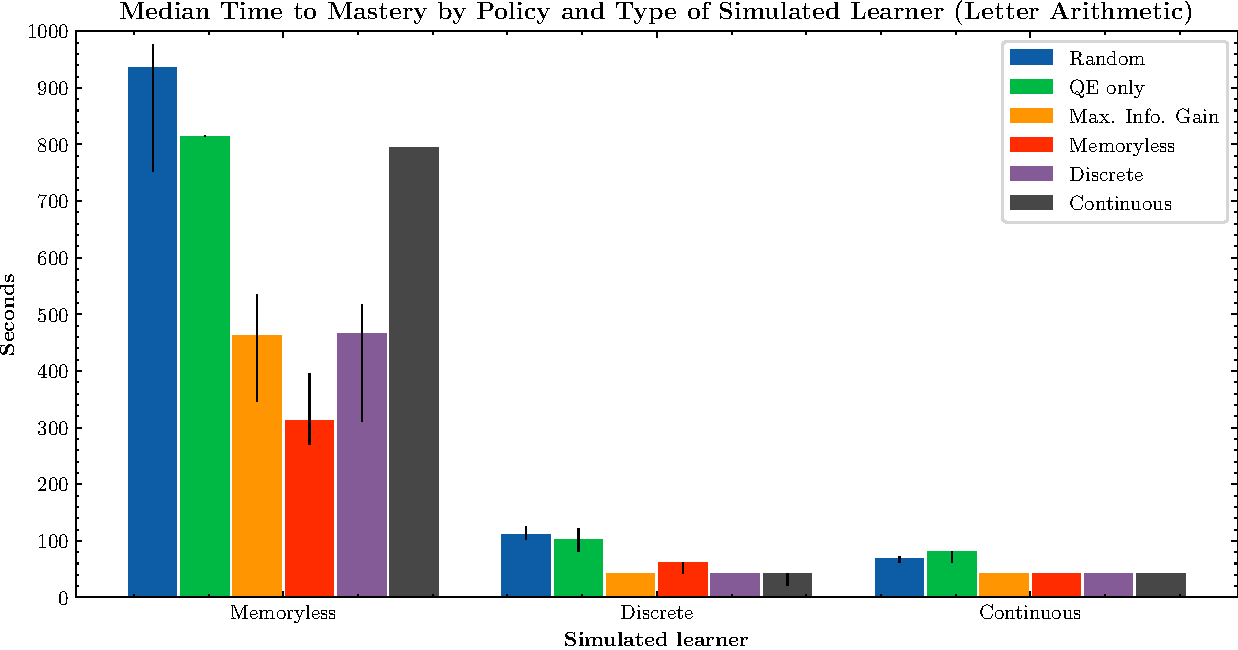
\includegraphics[width=\linewidth]{median-time-letter.pdf}
    \caption{Median time to mastery for the letter arithmetic task. The results are grouped for each simulated learner (x axis) showing the performance of the different policies. The error bars represent the bootstrapped 68\% confidence interval. Replication of figure 4 in the original paper.
    %The results are similar as well. Our results differ for the simulated memoryless learner which achieves a significantly better score for the memoryless planning model, and a worse score for the discrete memory planning model. Both the simulated learners with discrete memory and the continuous model achieve the same near minimum results with 42.0s, corresponding to two teaching phases with examples.
    }
    \label{fig:median-time}
\end{figure}

% TODO name discrete -> discrete memory everywhere


\subsubsection{Letter Arithmetic}

\begin{figure}
    \centering
    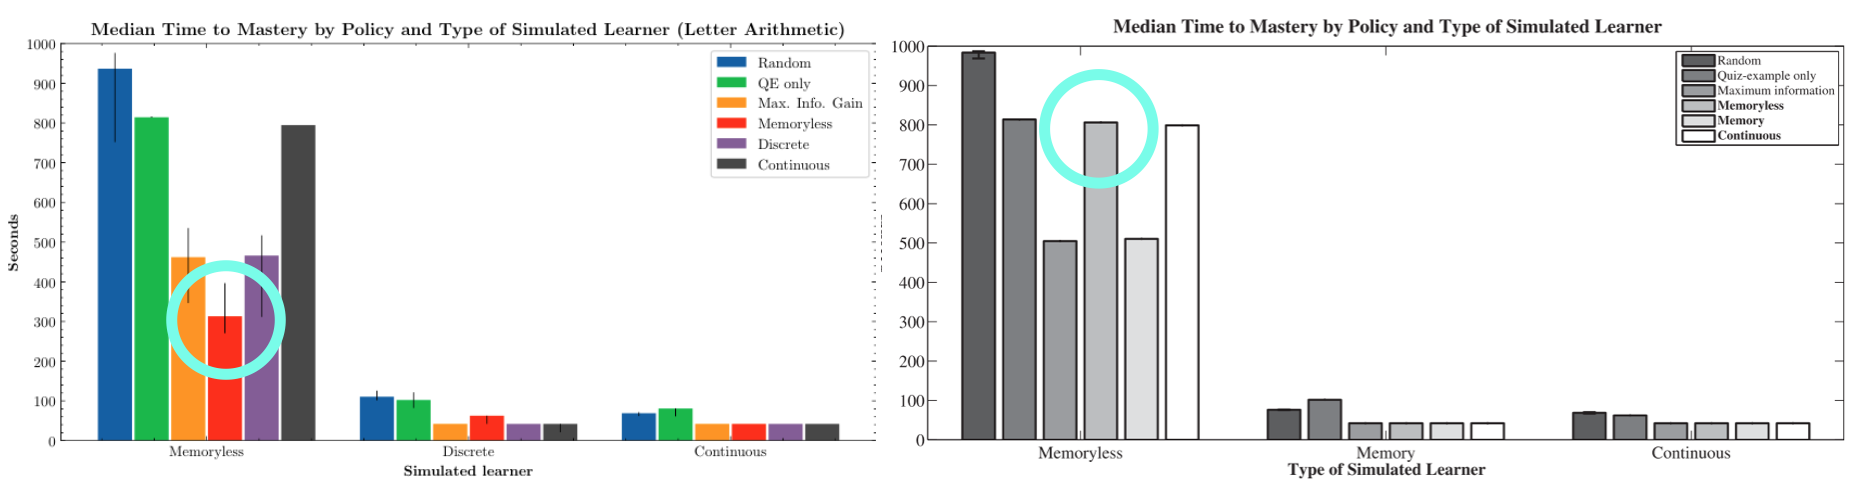
\includegraphics[width=\linewidth]{replication-diff-letter.png}
    \caption{Replication difference for the letter arithmetic task between our results (left) and the original data (right).
    }
    \label{fig:difference-t1}
\end{figure}


Our simulation results are shown in \autoref{fig:median-time}.
The overall results of the median time to mastery are very similar to the original paper.
A few differences exist, however. Eexact numbers for the original data are not available, so the values given below are approximated from Figure 4 of the original paper. 

Most notably, the result for the memoryless learner with the memoryless policy is different. It is lowest for the memoryless learner with 323.5s while the original authors reported a time around 800s. % TODO check number

The results for the other learners match pretty much the original data. 
The random policies differ slightly, albeit the difference is small.
The results with the POMDP policies for the discrete and continuous learner have all the same median at 42.0s except for the memoryless policy for the discrete learner (although its confidence interval comprises this value as well).
This applies to the maximum information gain policy as well, for which the time is equivalent to two rounds of example actions ($6 \cdot 7.0s$).

The failure rate of the different simulations, i.e. how many times a learning session was terminated after 40 rounds of teaching phases before the learner achieved mastery of the concept, are repoted in Table \ref{tab:failures-t1}. 
The results show that the memoryless learner consistently fails to learn the concept in nearly over 20\% of the cases.
It is highest with the continuous policy at 96\% and second highest for the random question-quiz only policy at 68\%. The median time to mastery is very similar though, even slightly lower with the continuous policy. The reason is that the policy starts to sample only the cheapest activity type (quiz) leading to the 
lower number even though it fails to teach properly.
The discrete memory learner only fails with the continuous policy in 26\% of the cases, while the continuous learner never fails to learn.
Although the information is not available in the original paper, since the median time to mastery is very close, we assume that the failures are similar as well.


\begin{table}
    \centering
    \small
    \begin{tabular}{l|rrr}
        \hline
        \textbf{Policy} & \multicolumn{2}{l}{\textbf{Failure rate with learner}} & \\
                        & Memoryless & Discrete memory & Continuous \\
        \hline
        Random          & 50\% & 0\% & 0\% \\
        Random QE only  & 68\% & 0\% & 0\% \\
        Max. Information Gain & 32\% & 0\% & 0\% \\
        \hline
        Memoryless      & 22\% & 0\% & 0\% \\
        Discrete memory & 18\% & 0\% & 0\% \\
        Continuous      & 96\% & 26\% & 0\% \\
        \hline
    \end{tabular}
    \caption{Failure rates over 50 simulations for each policy-learner pair. Failure is encountered when the concept is not learned after 40 teaching phases.}
    \label{tab:failures-t1}
\end{table}

When comparing the time to mastery for the two random policies, note that the random question-quiz only policy might achieve a lower number because the most expensive action is not used.
This can have a negative effect on the learning because for the full random policy, there is a $2/3$ chance of seeing evidence, while with QE only, only 50\% of the times new evidence is shown. 
This might explain the higher failure rate for the memoryless learner with the QE only model.

\begin{table}
\centering
\small
\begin{tabular}{lr|r}
\hline
\textbf{Model}  & \textbf{Planning Samples}    & \textbf{Mean computation time}  \\
\hline
Max. Info. Gain & 15     & 0.1s                  \\
\hline
Memoryless      & 7, 6            & 1.3s                  \\
Discrete memory & 8, 8            & 2.2s                  \\
Continuous      & 4, 3            & 1.2s                  \\
\hline
\end{tabular}
\caption{Planning times for different models for the letter arithmetic task. All learner models employ a planning horizon of 2.
%The two numbers in the samples refers to the number of samples at the first and second tree level. 
The max. information gain model only plans one step ahead.
%and tests all items with the example type.
}
\label{tab:times-t1}
\end{table}

\autoref{tab:times-t1} shows computation times for the different models across all learners. 
%Pre-planning is well below one minute in all cases. 
%However, only one or two paths are considered, as mostly example actions were planned which have no responses to adapt to. 
The online planning computation times are well below 3 seconds which was put forward as the threshold in the original paper. 
This means, we could increase the sample sizes and stay within the limit.
However, increasing the sample sizes did not produce very different results. We tested all increasing the sample size to 10 for all models and the results were the same for most of the simulations. The memoryless learner shows slightly different results for the memoryless and discrete memory policy, however, it lied still within the confidence interval of the results above.

Surely, computing power has increased since the publishing of the original paper, so it seems natural that more samples can be incorporated now (our trials were executed on a workstation with an Intel(R) Xeon(R) CPU E5-1650 v4 @ 3.60GHz and 32GB of RAM).

\begin{figure}
    \centering
    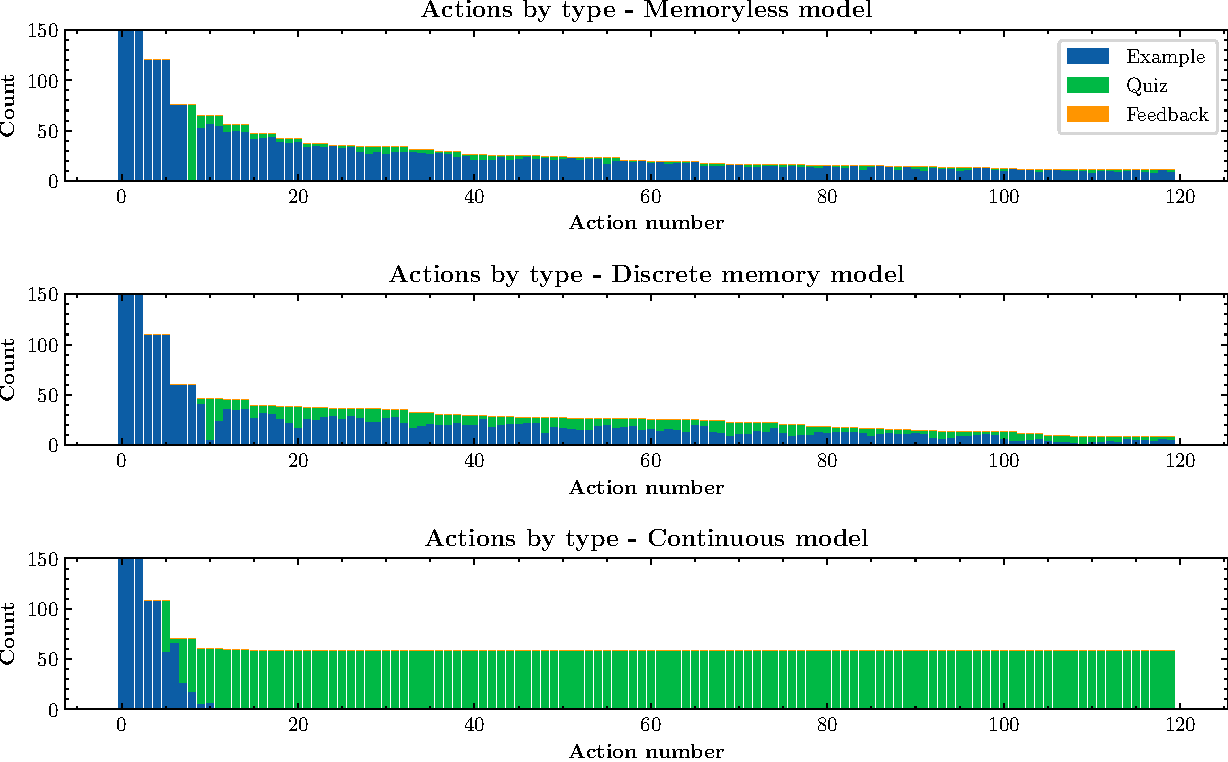
\includegraphics[width=\linewidth]{letter-actions-combi.pdf}
    \caption{Planned action type per step for each planning model for the letter arithmetic task. 
    %Example actions were predominantly chosen in the discrete models, while the continuous model planned mainly quiz actions after a few steps.
    }
    \label{fig:actions-t1}
\end{figure}

\autoref{fig:actions-t1} shows the teaching types planned for each model.
Both the memoryless model and the discrete memory model planned mainly example type actions.
Interestingly, both sampled a quiz type after eight and nine example types.
Afterwards, the discrete memory model employed more quizzes than the memoryless model.
The continuous model started with example type actions as well but gradually used more quiz type actions which were the only type used after action step 12.
No model planned feedback actions.


We provide detailed results and statistics in the supplementary section (see Table \ref{tab:results-t1}).

\subsubsection{Number game}

\begin{figure}[t]
    \centering
    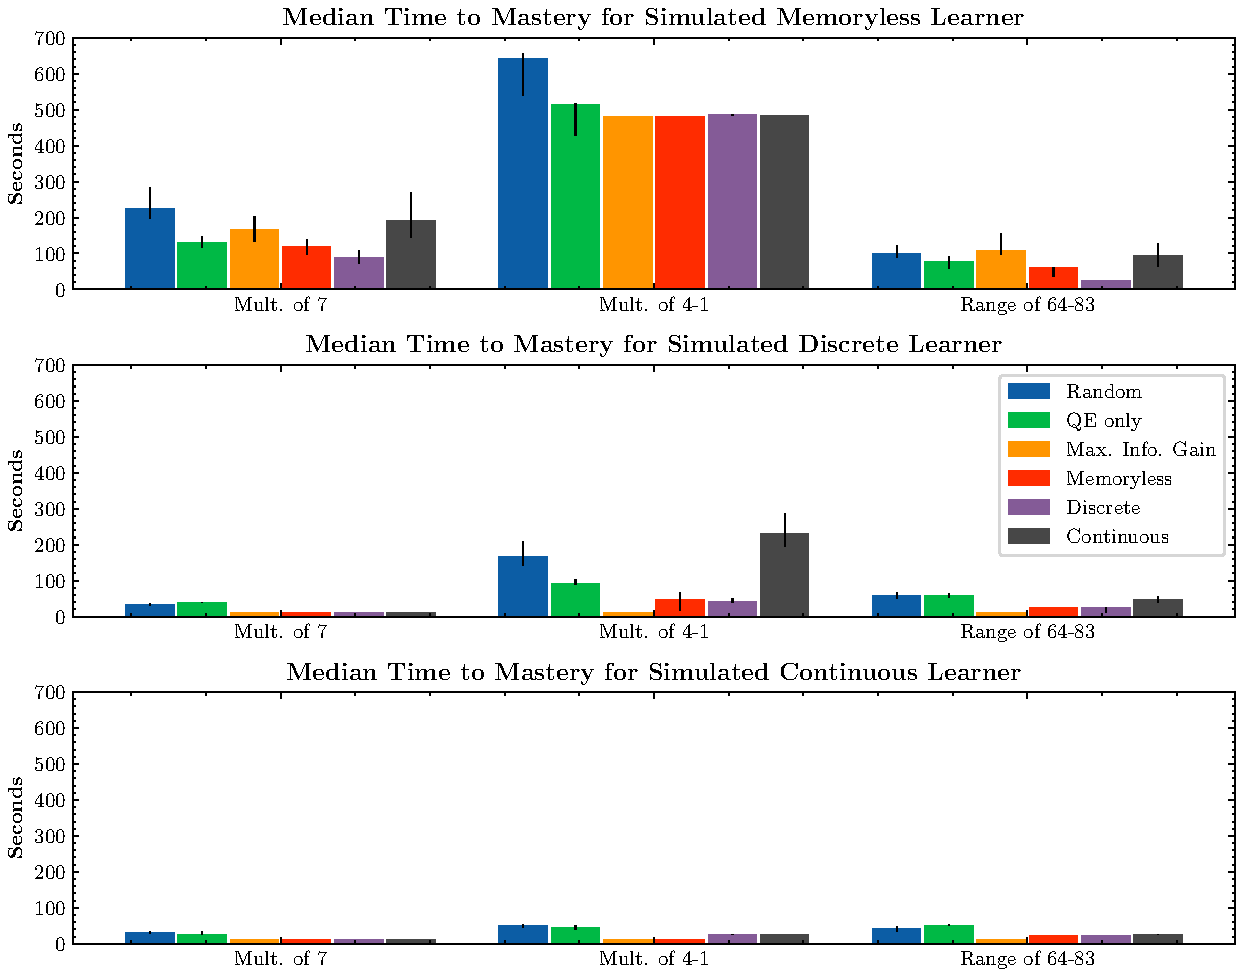
\includegraphics[width=\linewidth]{median-time-ng-combined.pdf}
    \caption{Median time to mastery for the number game separated for each simulated learner and grouped by task. 
    Error bars represent bootstrapped 68\% confidence intervals. 
    Comparable to figure 9 of the original paper.}
    \label{fig:median-time-ng}
\end{figure}


\begin{figure}
    \centering
    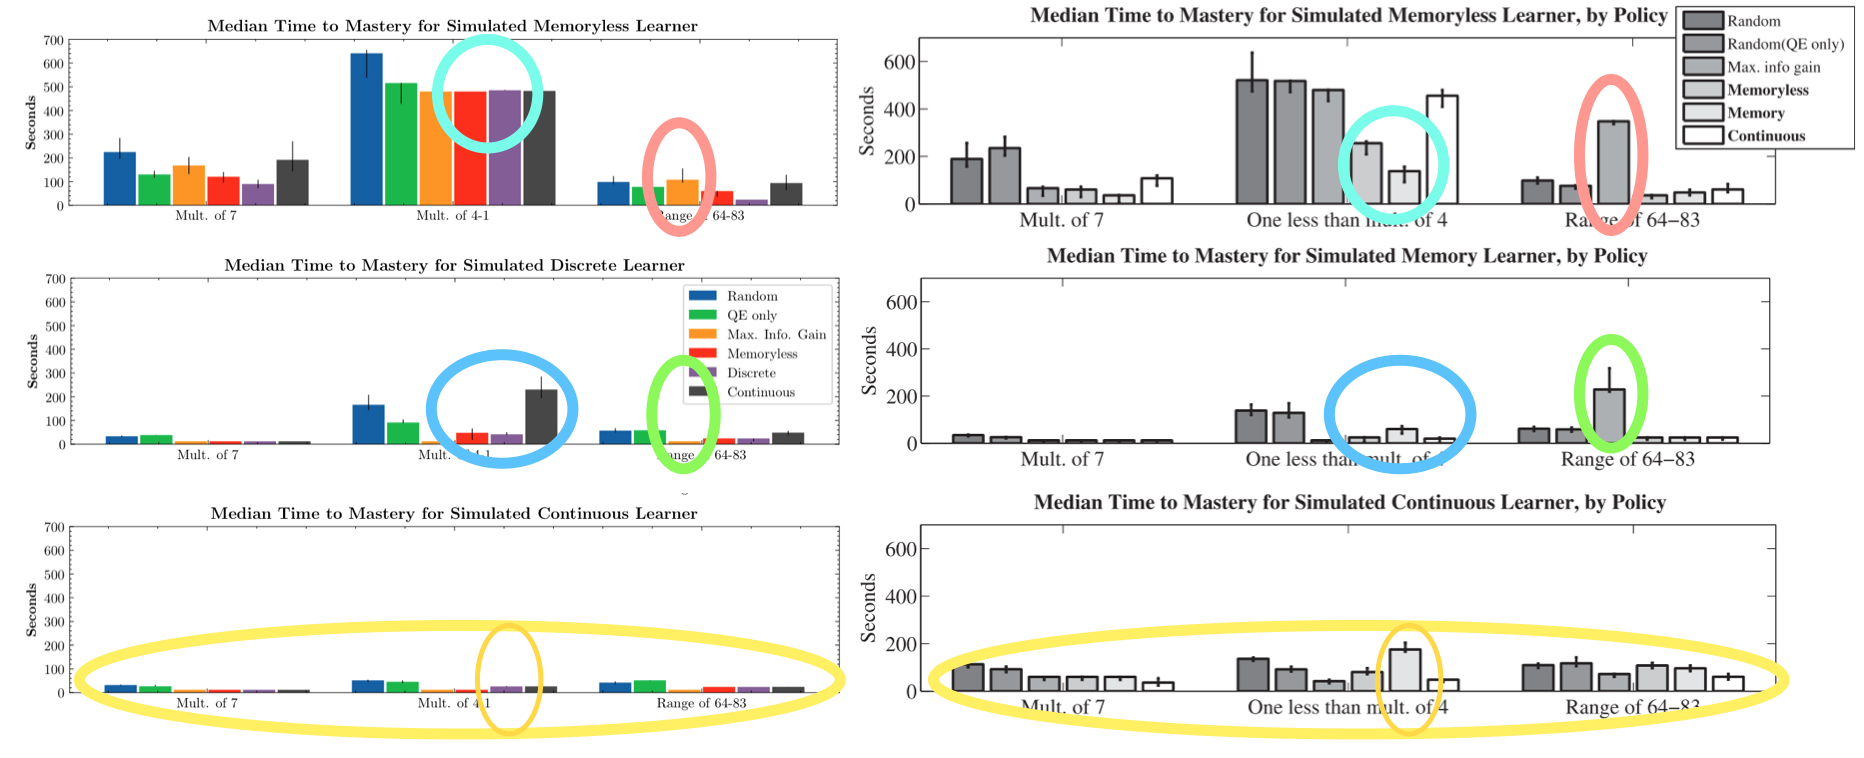
\includegraphics[width=\linewidth]{replication-diff-number-game.png}
    \caption{Replication difference for the number game between our results (left) and the original data (right).
    }
    \label{fig:difference-t2}
\end{figure}


Our results are shown in figure \ref{fig:median-time-ng}. 
The overall structure of the results appear similar to the original results, especially for the task multiples of 7. 
In the others, there are a few notable differences in our data. 

For the simulated memoryless learner (top chart), our results for the target \textit{multiples of 7} are slightly higher and not clearly better than the random policies while their relative performance matches the previously reported results.
For the target \textit{multiples of 4 minus 1}, our results with the memoryless planner and the discrete memory planner differ significantly. 
Our simulations resulted in a median time to mastery of ~480s for both which was reported as ~250s and ~150s in the previous work. 
% TODO exact numbers: worth it to read from small charts??
As a results, no planner exhibits a high performance while previously, the discrete planners resulted in low teaching times.
In the target \textit{Range of 64-83}, we find the maximum information gain policy performs comparable to the continuous policy at 108s while it performed significantly worse than the other planners at ~350s in the original results.

For the simulated discrete memory learner (middle row), with the target \textit{multiples of 4 minus 1}, our continuous planner resulted in a significantly worse performance than all other policies which performed remarkable in the previous paper.
For target \textit{Range of 64-83}, our maximum information gain policy achieves a very high performance with 12s, while in the original results, it was significantly worse than all the other policies with over 200s.

For the simulated continuous learner, we find it to perform significantly better with all target and with all policies, achieving the best results among the different learners allowing no distinguishing between the planners' performance. 
In the original work, the continuous learner was outperformed in many cases by the discrete memory learner and even sometimes the memoryless learner.

In general, we note that our results do not follow a clear line in comparison to the original data.
The best policy for a combination is often different in our simulations even if the differences are not large and the overall image is comparable to the previous work.


\begin{table}
    \centering
    \small
    \begin{tabular}{l|rrr|rrr|rrr}
        \hline
        \textbf{Policy} & \multicolumn{3}{l|}{\textbf{Multiples of 7}}  & \multicolumn{3}{l|}{\textbf{Mult. of 4 minus 1}} &  \multicolumn{3}{l}{\textbf{Range 64-83}} \\
                        & Mless & Mem. & Cont. & Mless & Mem. & Cont. & Mless & Mem. & Cont. \\
        \hline
        Random          & 12\% & 0\% & 0\% &            54\% & 2\% & 0\% &      2\% & 0\% & 0\% \\
        QE only         & 6\% & 0\% & 0\% &            54\% & 2\% & 0\% &      0\% & 0\% & 0\% \\
        Max Info Gain & 16\% & 0\% & 0\% &             72\% & 6\% & 0\% &      6\% & 0\% & 0\% \\
        \hline
        Memoryless      & 4\% & 0\% & 0\% &            70\% & 0\% & 0\% &      0\% & 0\% & 0\% \\
        Memory          & 4\% & 0\% & 0\% &            70\% & 0\% & 0\% &      0\% & 0\% & 0\% \\
        Continuous      & 28\% & 0\% & 0\% &           68\% & 18\% & 0\% &       0\% & 0\% & 0\% \\
        \hline
    \end{tabular}
    \caption{Failure rates over 50 simulations for the number game tasks. }
    \label{tab:failures-t2}
\end{table}

\autoref{tab:failures-t2} shows the failure rates for the second experiment. 
We note similar results as in the first experiment: The memoryless learner fails to learn in some cases, especially for the target \textit{multiples of 4 minus 1}. In fact, the failure rates are very similar across all planners.
In that task, also the discrete memory learner fails to learn with the random, maximum information gain and continuous policies.
The failure rates are somewhat lower though than in the first experiment.
The continuous learner never fails to learn.


\begin{table}
\centering
\small
\begin{tabular}{lr|r}
\hline
\textbf{Model}  & \textbf{Samples}    & \textbf{Mean computation time}  \\
\hline
Max. Info. Gain & 100             & 0.2s                  \\
\hline
Memoryless      & 6, 8            & 3.7s                  \\
Discrete        & 6, 6            & 2.4s                  \\
Continuous      & 6, 6, 8            & 21.92s                  \\
\hline
\end{tabular}
\caption{Planning times for different models for the number game.}
\label{tab:times-t2}
\end{table}

The computation times are reported in table \ref{tab:times-t2}. We see that the computation times are now significantly higher than in the first experiment and they are close or bigger than the threshold of 3s. 
Especially the continuous policy showed a mean computation time of more than 20s because it was planning three horizons into the future.
%%% Lukas: In the first task the runtime was never an issue, so I didnt do the cutoff after 3s like they described in the paper. Now I'm thinking for this task it could produce some differences - however overall, for the continuous model the results are close in most cases and rather worse despite the possibly larger search. What do you reckon?
The higher computation times make sense considering that the state space is around 7 times larger than in the letter arithmetic task\footnote{The precomputation times were sometimes significantly high for the number game, depending on the number of quizzes it sampled in the first 20 steps. This resulted in some cases in over 5,000 paths to be precomputed and a runtime of more than 10 hours. In most cases though, the number of evaluated paths was below 10 and done in few minutes.}.
Note though that we invested less effort into making the computations efficient for the number game.

\begin{figure}
    \centering
    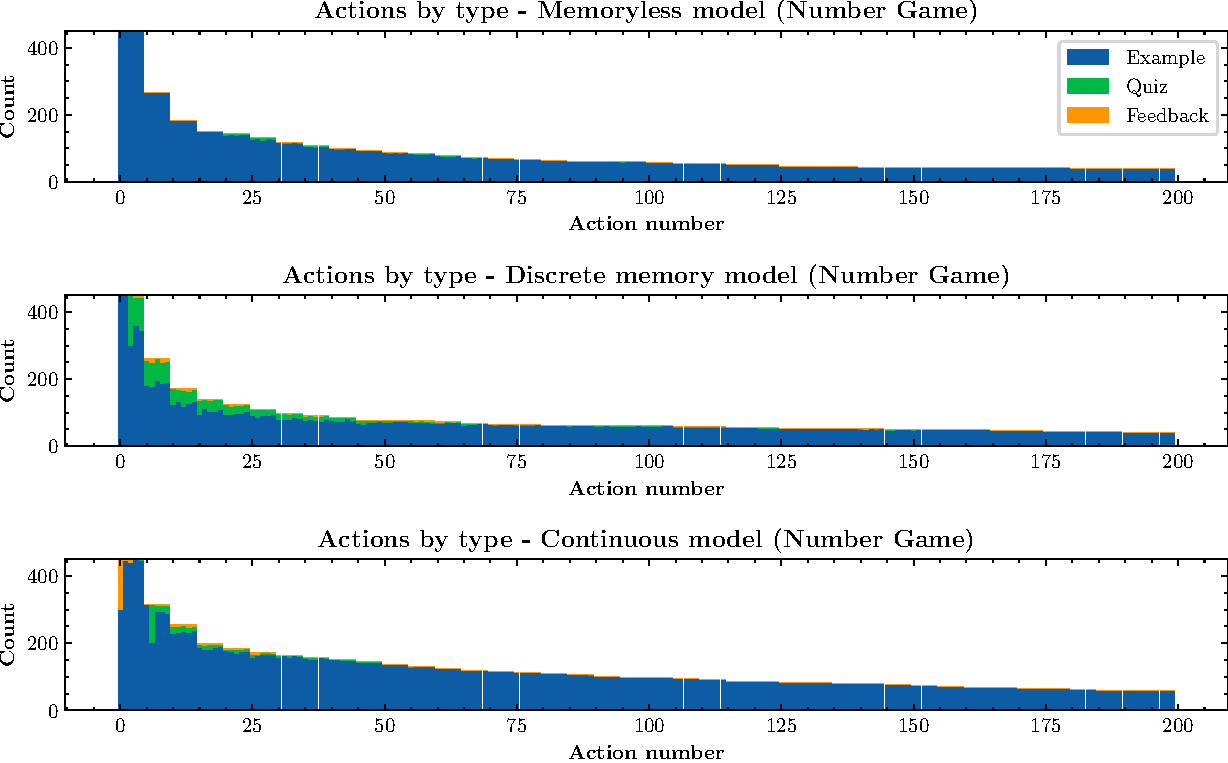
\includegraphics[width=\linewidth]{ng-actions-combi.pdf}
    \caption{Planned action type per step for each planning model for the number game. 
    %Example actions were predominantly chosen.
    }
    \label{fig:actions-t2}
\end{figure}

Finally, Figure \ref{fig:actions-t2} shows the sampled teaching types for the different models, combined for all three tasks.
Recall that in the number game, the cheapest action type was the example action.
We notice that it is strongly dominated by example actions in all planners.
The memoryless model chose feedback actions extremely rarely. 
The discrete memory and the continuous model chose feedback actions slightly more as well as a few quiz actions.

Again, detailed results and statistics are provided in the supplementary section.
% TODO

\subsection{Implementation}

We implemented the model in Python 3, using Numpy to perform as many of the calculations in vectorized form as possible. 
Simulations are run in parallel to reduce the needed execution time. 
Reproducibility is achieved by using fixed seeds for the random number generators in Python and Numpy. 
The code is publicly available on GitHub\footnote{https://github.com/luksurious/faster-teaching/}. 
All possible execution modes are configurable via command-line arguments which also allows a manual learning mode for diagnosis. 

All simulations were executed on Ubuntu 18.04 and 19.10 with Python 3.7.5.

To improve performance, the belief update is always performed according to the two actions types described above (separate refinement and evidence updates) as opposed to performing the full Bayesian belief update according to the generic formula. 
Further, the planning algorithm is slightly improved to stop the iteration over possible observations if the current cost of the action is already higher than the currently known best value.
% Note though, that the code for the letter arithmetic task is more optimized than the code for the number game.

Similar to the particle filter handling in the continuous model where the particles are recreated if the weights are too small, the belief for the discrete models are reset to the initial belief for inconsistent responses leading to beliefs with zero probability on all concepts.

In the random policy, to achieve a sensible baseline, we ensure that the same item is not used in a single teaching phase.

Since we did not perform a user study, limiting the calculations using a time limit have not been implemented. 


\section{Discussion}

\subsection{Results}
We were able to partially replicate the results reported by Rafferty et al. for the simulated learners.
Indeed, the overall picture remains the same but we found small differences that might lead to a slightly different evaluation.

We encountered two main differences in our replication. First, in the letter arithmetic task, the memoryless policy performed much better for the memoryless learner. Intuitively this makes sense because it is matching the psychological model between the planner and learner.
Second, in the number game, our maximum information gain policy achieved reasonable performance and performed at least as good as one of the other learner models.

Additionally, when evaluating the learner models, our results provide extra information regading the failure rates.
The time alone can be misleading as it might mask failure rates with cheap actions as it is the case with the continuous planner in the first task. 
From this analysis we found that the simulated memoryless learner often fails to learn the concept and as such it seems not a very plausible model for human concept learning because in the original paper, the human learners seemed to have learned the letter arithmetic task correctly.
On the other side, the continuous policy most often led to failures in the learners, indicating that it is not well suited for different types of learners.
This can also be seen from the types of actions sampled. In the letter arithmetic task, it chose only quiz actions which fails to teach anything and resulted in the high failure rate for the memoryless learner.
This is in line with the analysis by Rafferty et al. that the continuous policy overestimates the learning capabilities and might not discover a divergence between the belief and the true state.

%In many cases, the difference between the POMDP models are not large, so considering the computational requirements, it seems that the more conservative and simple memoryless model would be a good choice for practical applications. 
%Overall, the memoryless model achieves the best scores considering the different types of learners together.

Certainly, the random policies were not good teachers.
However, the policy based on the maximum information gain achieved comparable results to the other POMDP models, while mostly failing in the original paper. 
% We did not find it to be failing as in the original paper.
% Since it also employs the continuous belief model inside to trace the state of the learner, we argue that it should still be considered as a POMDP policy rather than a baseline.
%Considering the computational costs of the forward search planning, it appears to be a reasonable and low-cost approach.
% Even so, the computation times with the other policies is not comparable because it only searches over a horizon of one instead of two or three.
Since it also employs the continuous belief model inside to trace the state of the learner, it would be interesting to see whether reducing the horizon of the other models leads to similar performance (with better runtimes) and if the maximum information gain policy can be further improved by increasing the horizon.

In the number game, we find it surprising that the horizon for the continuous model was set to three with similar sample sizes as the discrete models that only search two levels. 
This is in contrast to the settings of the first task where all models used the same horizon and the continuous policy sampled fewer items.
Considering that the state space is around 7 times larger in the number game than in the letter arithmetic tasks, it is counter-intuitive to largely increase the search space.
As a result, we show that the computation times in this case is significantly increased, well above a reasonable threshold of three seconds.


% model discussion

The two discrete models (memoryless model and model with memory) might be defined in a too simple way to reflect human learning because the transition probability to a new consistent state is not dependent on the current state.
%Especially in the memoryless model, the transitions to new states is a random guess based only on the current information. 
In an MDP, states can contain information about the history and transitions often depend on the current state, e.g. favoring transitions to states that are closer to the current state. 
The same can be applied here: as the current state contains information about the previous action, we can exploit this information without keeping an explicit history by assigning higher probability to states with less distance to the current state. 
In the letter arithmetic task, the distance can be measured for instance by the number of necessary pairwise changes to move from one state to another. 
We argue that this also better reflects human learning. 
%Integrating this into the learner model can improve the performance significantly for cases with related states.
%(see \autoref{sec:supp}) and renders the memoryless model actually usable. 
In larger domains, it would also make convergence to the target state more likely as the implicit history inside the state is better utilized.

Additionally, the discrete model with memory assumes a perfect memory. 
It seems plausible that this is not always the case for human learners and might be a too strong assumption. 
However, if different memory state possibilities were integrated into the model, the state space would increase significantly, reducing it's tractability. 
Nevertheless, this could be a reason for the high transition noise determined for this learner model in the letter arithmetic task.


% task discussion

The results show that for a strong learner, the planning model is not very important as all achieve high performance. For a weaker learner, our simulations show that a similarly policy with weaker learning assumptions fits best.
%While it was possible to show that the model is able to plan better than a random model, it seems too simple to really evaluate the the models as the baseline using only example actions based on the maximum information gain achieves the same results in terms of median time to mastery as the more sophisticated POMDP models.

The letter arithmetic task might be too simple to draw conclusions from. This is in line with the second experiment in the original paper which reported even performance across all POMDP policies (including the maximum information gain policy).
In the number game, the results are more differentiated but still it is not possible to draw clear conclusions about the suitability of a policy and whether they are superior to the maximum information gain policy.


%Yet, already for this simple problem, the planning horizon was very short because the computational requirements increase exponentially and increasing the horizon makes it unusable in a live setting.


\subsection{Framework}
%%% Lukas: I might be discussing too much?
One key to implementing the models efficiently is to not use the explicit Bayesian formula for belief updates but instead treat the belief update separately for inferring the learner's previous state and for calculating transitions based on new evidence.


% framework discussion

% teaching goal, cost definitions
Defining the teaching goal and associated rewards or costs is a critical part in this framework.
Focusing on shortest time and associating the average time to process an action type nearly eliminated one of the teaching types (feedback type) in our simulations, presumably due to the high costs associated. 
It was shown that the continuous model converges to the cheapest action type and the differences in costs between the first and second task resulted in a very different behavior of the model.
As the main planning decision, as stated in the original paper, can be seen as deciding between teaching new content (examples) versus inferring the learner's state (quizzes), defining the cost function in the current way does not seem to facilitate this decision well enough. 


% leaf estimation
Similarly, the value for estimating leaf nodes needs more evaluation. 
The scale of the formula postulated needs to be scaled appropriately to the state space and corresponding changes in success probability from teaching actions. 
Otherwise, the forward search could lead to mainly choosing the cheapest action if the success probability of the correct concept is too small in comparison.
%%% Lukas: Should I add an example? It is a rather simple calculation but a bit tricky to explain in short words.
%\footnote{A simple calculation. Assume the cheapest action type quiz has a cost associated of 4, this means the success probability in the leaf calculation is scaled by 40. When choosing a quiz, the learner's state does not change. .... p(true)= 1e-6. With quiz 1 horizon, val = 4+40*1e-6=4.00004. Example costs 5 and pushes to true concept, p(true)=1e-5. Val = 5+40*1e-5=5.0004. With uniform observation probability. this actually happens in the number game for the most unlikely concept (multiples of 4 minus 1) if the values of the first task are taken}
Hence, it would be interesting to see if the estimation of leaf nodes correspond to the true values of the states in the experiments.

% future
%These costs are highly important but remain fixed for all participants even though it seems plausible that different learners exhibit different learning times. 
%In a real experiment, it would be interesting to see if adapting the costs of the actions to the historical data taken by that user would adapt better to the individual and possibly make feedback types more attractive to use. 

%Possibly adapt the estimation function accordingly to fit the data.
%Similar data and user-based adaptation could be performed for the noise parameters to adapt to the individual learners.

% assessment phase, determining goal state
% how is it done in "regular POMDPs"? shouldnt either the belief determine if the agent stops (i.e. cont. model stops even if not learned), or it is a separate action/observation which would then be integrated into the model and belief updates??
Having a separate assessment phase whose purpose is solely to determine if the teaching is finished, and not using the responses to tune the belief, appears counter-intuitive. 
This results in a few cases where the teacher is not able to determine the wrong hypothesis of the learner when the belief diverges from the true state, and no quiz actions are planned to validate the belief. 
In a human experiment, the assessment phase might also give additional information about the concept to be learned (e.g. in the number game) as learners might assume that some should be from within the concept.
Integrating the assessment phase into the planning model could alleviate these issues and enforce more regular "sanity checks" as otherwise the teaching would not terminate.



% formulation as POMDP still interesting, although concrete tasks and learner models seem in need of adjustment



\section{Conclusion}
Formulating teaching as a POMDP is certainly an interesting approach that allows to use sophisticated planning algorithms with cognitive learner models.
% We replicated the work by Rafferty et al. with some differences.
% , and also clarified the formulation in a more rigorous way.
% In the proposed context of concept learning, there is no clear differentiation in terms of performance between the different learner models and the policy based on the continuous model with maximum information gain.
% For further application, we argue that the optimization goal and cost definition should be formulated differently to produce be more robust and address the issue of learning failure.
% Further, 
It would be interesting to extend this work to apply it to real-world teaching problems (e.g. second language learning), and through this  replication, we hope to facilitate research in this direction. % by providing an extended description and a free implementation of the Faster Teaching's algorithm.

\section{Acknowledgements}
We would like to thank Anna Rafferty (the first author of the original paper) for answering our numerous questions and sharing her implementation with us.

\section{Author contributions}
Planning and discussion of the implementation incl. clarifications on the original method was shared equally between L. Brückner and A. Nioche. The implementation itself was done by L. Brückner.
